% Practice Test 15 — Florida Edition
% Questions: 30 (20 MC + 10 SA)
% Generated by scripts/generate_practice_tests.py

\begin{practiceQuestion}{1-3-q07}{mc}
\begin{questionText}
The table shows hours worked and money earned. What is $k$ and what does it mean?

\begin{center}
\begin{tabular}{|c|c|}
\hline \textbf{Hours} & \textbf{Earnings (\$)} \\ \hline $\frac{1}{2}$ & $\$6$ \\ $1$ & $\$12$ \\ $3$ & $\$36$ \\ \hline
\end{tabular}
\end{center}
\end{questionText}
\choiceA{$k = 6$; earns $\$6$ per half hour}
\choiceB{$k = 12$; earns $\$12$ per hour}
\choiceC{$k = 36$; earns $\$36$ per $3$ hours}
\choiceD{$k = 3$; works $3$ hours per $\$36$}
\correctAnswer{B}
\explanation{$k = \frac{6}{0.5} = 12$ or $\frac{12}{1} = 12$ or $\frac{36}{3} = 12$. The unit rate is $\$12$ per hour.}
\end{practiceQuestion}

\begin{practiceQuestion}{1-6-q03}{mc}
\begin{questionText}
A car travels $210$ miles on $6$ gallons of gas. How far can it go on $10$ gallons?
\end{questionText}
\choiceA{$300$ miles}
\choiceB{$330$ miles}
\choiceC{$350$ miles}
\choiceD{$360$ miles}
\correctAnswer{C}
\explanation{Unit rate: $210 \div 6 = 35$ mpg. On $10$ gallons: $35 \times 10 = 350$ miles.}
\end{practiceQuestion}

\begin{practiceQuestion}{2-1-q18}{mc}
\begin{questionText}
Mia scored $85\%$ on a test with $60$ questions. How many questions did she answer correctly?
\end{questionText}
\choiceA{$48$}
\choiceB{$50$}
\choiceC{$51$}
\choiceD{$54$}
\correctAnswer{C}
\explanation{$85\% = 0.85$. Multiply: $0.85 \times 60 = 51$ questions correct.}
\end{practiceQuestion}

\begin{practiceQuestion}{2-2-q18}{mc}
\begin{questionText}
A classroom has $28$ students. $7$ of them wear glasses. What percent wear glasses?
\end{questionText}
\choiceA{$20\%$}
\choiceB{$25\%$}
\choiceC{$28\%$}
\choiceD{$35\%$}
\correctAnswer{B}
\explanation{$\frac{7}{28} = \frac{p}{100}$. Cross-multiply: $28p = 700$. Divide: $p = 25\%$.}
\end{practiceQuestion}

\begin{practiceQuestion}{2-6-q24}{sa}
\begin{questionText}
What principal do you need to deposit at $4\%$ simple interest to earn $\$360$ in $3$ years?
\end{questionText}
\correctAnswer{$\$3{,}000$}
\explanation{$360 = P \times 0.04 \times 3$ → $360 = 0.12P$ → $P = \$3{,}000$.}
\end{practiceQuestion}

\begin{practiceQuestion}{2-7-q15}{mc}
\begin{questionText}
A chemist expected to collect $75$ mL of solution but collected $80$ mL. What is the percent error (rounded to the nearest tenth)?
\end{questionText}
\choiceA{$5\%$}
\choiceB{$6.3\%$}
\choiceC{$6.7\%$}
\choiceD{$7.5\%$}
\correctAnswer{B}
\explanation{$\frac{|75 - 80|}{80} \times 100 = \frac{5}{80} \times 100 = 6.25 \approx 6.3\%$.}
\end{practiceQuestion}

\begin{practiceQuestion}{3-2-q24}{sa}
\begin{questionText}
A football team has the following plays: gain $7$ yards, lose $3$ yards, lose $5$ yards, gain $2$ yards. What is the net yardage?
\end{questionText}
\correctAnswer{$1$ yard}
\explanation{$7 + (-3) + (-5) + 2 = 1$. Gains: $7 + 2 = 9$. Losses: $3 + 5 = 8$. Net: $9 - 8 = 1$ yard gained.}
\end{practiceQuestion}

\begin{practiceQuestion}{3-3-q20}{sa}
\begin{questionText}
What is $(-8) - (-15)$?
\end{questionText}
\correctAnswer{$7$}
\explanation{$(-8) - (-15) = (-8) + 15 = 7$.}
\end{practiceQuestion}

\begin{practiceQuestion}{4-4-q28}{gmc}
\begin{questionText}
The rectangle below has the given area. Which pair of dimensions is correct?

\begin{center}
\begin{tikzpicture}[scale=0.7]
  \draw[thick, fill=funBlue!10] (0,0) rectangle (6,2.5);
  \node at (3,1.25) {Area $= 10x + 35$};
  \node[left] at (0,1.25) {?};
  \node[below] at (3,0) {?};
\end{tikzpicture}
\end{center}
\end{questionText}
\choiceA{Width $= 5$, Length $= 2x + 7$}
\choiceB{Width $= 10$, Length $= x + 35$}
\choiceC{Width $= 5$, Length $= 2x + 35$}
\choiceD{Width $= 2$, Length $= 5x + 35$}
\correctAnswer{A}
\explanation{Factor: $10x + 35 = 5(2x + 7)$. So the width is $5$ and the length is $2x + 7$.}
\end{practiceQuestion}

\begin{practiceQuestion}{4-5-q24}{sa}
\begin{questionText}
Write two linear expressions whose sum is $7x + 2$.
\end{questionText}
\correctAnswer{Answers vary, e.g., $(4x + 1)$ and $(3x + 1)$}
\explanation{Any two expressions whose like terms add to $7x + 2$ work. For example, $(4x + 1) + (3x + 1) = 7x + 2$.}
\end{practiceQuestion}

\begin{practiceQuestion}{5-3-q17}{mc}
\begin{questionText}
Solve $-3(2n + 4) = -24$.
\end{questionText}
\choiceA{$n = 6$}
\choiceB{$n = -2$}
\choiceC{$n = 2$}
\choiceD{$n = 4$}
\correctAnswer{C}
\explanation{Divide by $-3$: $2n + 4 = 8$. Subtract $4$: $2n = 4$. Divide by $2$: $n = 2$. Check: $-3(2(2)+4) = -3(8) = -24$ \checkmark.}
\end{practiceQuestion}

\begin{practiceQuestion}{5-4-q09}{mc}
\begin{questionText}
Solve $1.2x + 0.8 = 4.4$.
\end{questionText}
\choiceA{$x = 3$}
\choiceB{$x = 4.33$}
\choiceC{$x = 3.6$}
\choiceD{$x = 2.5$}
\correctAnswer{A}
\explanation{Subtract $0.8$: $1.2x = 3.6$. Divide by $1.2$: $x = 3$. Check: $1.2(3) + 0.8 = 3.6 + 0.8 = 4.4$ \checkmark.}
\end{practiceQuestion}

\begin{practiceQuestion}{5-5-q15}{mc}
\begin{questionText}
A student needs at least $70$ points to pass a test. She earns $4$ points per question and has $10$ bonus points. Which inequality finds the minimum number of questions $q$ she must answer?
\end{questionText}
\choiceA{$4q + 10 > 70$}
\choiceB{$4q + 10 \geq 70$}
\choiceC{$4q - 10 \geq 70$}
\choiceD{$10q + 4 \geq 70$}
\correctAnswer{B}
\explanation{Score $= 4q + 10$, needs at least $70$: $4q + 10 \geq 70$.}
\end{practiceQuestion}

\begin{practiceQuestion}{5-6-q25}{sa}
\begin{questionText}
Solve $7x - 3 \geq 18$. Give the smallest integer that is a solution.
\end{questionText}
\correctAnswer{$x = 3$}
\explanation{Add $3$: $7x \geq 21$. Divide by $7$: $x \geq 3$. The smallest integer solution is $3$.}
\end{practiceQuestion}

\begin{practiceQuestion}{6-2-q26}{gmc}
\begin{questionText}
The original drawing below uses scale $1$ cm $= 10$ m. You are asked to redraw the rectangle at scale $1$ cm $= 5$ m. What will the new dimensions be?

\begin{center}
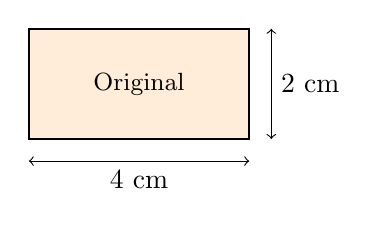
\begin{tikzpicture}[scale=0.7]
  \draw[thick,fill=orange!15] (0,0) rectangle (4,2);
  \draw[<->] (0,-0.4) -- (4,-0.4);
  \node[below] at (2,-0.4) {$4$ cm};
  \draw[<->] (4.4,0) -- (4.4,2);
  \node[right] at (4.4,1) {$2$ cm};
  \node at (2,1) {\small Original};
\end{tikzpicture}
\end{center}
\end{questionText}
\choiceA{$2$ cm by $1$ cm}
\choiceB{$4$ cm by $2$ cm}
\choiceC{$8$ cm by $4$ cm}
\choiceD{$20$ cm by $10$ cm}
\correctAnswer{C}
\explanation{Scale ratio: $\frac{10}{5} = 2$. New dimensions: $4 \times 2 = 8$ cm by $2 \times 2 = 4$ cm.}
\end{practiceQuestion}

\begin{practiceQuestion}{6-4-q22}{sa}
\begin{questionText}
A triangle has sides $11$, $13$, and $20$. Does it satisfy the triangle inequality?
\end{questionText}
\correctAnswer{Yes}
\explanation{$11 + 13 = 24 > 20$ \checkmark, $11 + 20 = 31 > 13$ \checkmark, $13 + 20 = 33 > 11$ \checkmark. All three checks pass.}
\end{practiceQuestion}

\begin{practiceQuestion}{6-5-q03}{mc}
\begin{questionText}
You slice a cone with a horizontal cut parallel to its base. What shape is the cross-section?
\end{questionText}
\choiceA{A circle smaller than the base}
\choiceB{A circle the same size as the base}
\choiceC{A triangle}
\choiceD{A rectangle}
\correctAnswer{A}
\explanation{A horizontal cut through a cone parallel to the base produces a circle smaller than the base. The higher you cut, the smaller the circle.}
\end{practiceQuestion}

\begin{practiceQuestion}{6-6-q06}{mc}
\begin{questionText}
Which pair of angles are supplementary?
\end{questionText}
\choiceA{$45°$ and $45°$}
\choiceB{$60°$ and $30°$}
\choiceC{$110°$ and $70°$}
\choiceD{$100°$ and $100°$}
\correctAnswer{C}
\explanation{Supplementary angles sum to $180°$. $110 + 70 = 180$ \checkmark. The others: $45 + 45 = 90$, $60 + 30 = 90$, $100 + 100 = 200$. Only C works.}
\end{practiceQuestion}

\begin{practiceQuestion}{7-1-q15}{mc}
\begin{questionText}
The diameter of a pizza is $16$ inches. What is the radius?
\end{questionText}
\choiceA{$4$ inches}
\choiceB{$8$ inches}
\choiceC{$16$ inches}
\choiceD{$32$ inches}
\correctAnswer{B}
\explanation{$r = d \div 2 = 16 \div 2 = 8$ inches.}
\end{practiceQuestion}

\begin{practiceQuestion}{7-5-q21}{sa}
\begin{questionText}
A cereal box is $25$ cm tall, $18$ cm wide, and $5$ cm deep. How much cardboard is needed to make the box?
\end{questionText}
\correctAnswer{$1330$ cm$^2$}
\explanation{$SA = 2(25 \times 18) + 2(25 \times 5) + 2(18 \times 5) = 900 + 250 + 180 = 1330$ cm$^2$.}
\end{practiceQuestion}

\begin{practiceQuestion}{7-6-q24}{sa}
\begin{questionText}
A planter box is $3$ ft long, $1.5$ ft wide, and $2$ ft deep. How many cubic feet of soil are needed to fill it?
\end{questionText}
\correctAnswer{$9$ ft$^3$}
\explanation{$V = 3 \times 1.5 \times 2 = 9$ ft$^3$.}
\end{practiceQuestion}

\begin{practiceQuestion}{7-7-q13}{mc}
\begin{questionText}
A paint can is a cylinder with radius $7$ cm and height $20$ cm. What is the surface area of the paint can? Use $\pi \approx \frac{22}{7}$.
\end{questionText}
\choiceA{$308$ cm$^2$}
\choiceB{$880$ cm$^2$}
\choiceC{$1{,}188$ cm$^2$}
\choiceD{$616$ cm$^2$}
\correctAnswer{C}
\explanation{$SA = 2\pi r^2 + 2\pi rh = 2 \times \frac{22}{7} \times 49 + 2 \times \frac{22}{7} \times 7 \times 20 = 308 + 880 = 1{,}188$ cm$^2$.}
\end{practiceQuestion}

\begin{practiceQuestion}{8-1-q01}{mc}
\begin{questionText}
A school has $800$ students. The principal surveys $50$ students about their favorite subject. What is the population?
\end{questionText}
\choiceA{The $50$ surveyed students}
\choiceB{All $800$ students in the school}
\choiceC{The principal}
\choiceD{The students who like math}
\correctAnswer{B}
\explanation{The population is the entire group you want to study — all $800$ students.}
\end{practiceQuestion}

\begin{practiceQuestion}{8-3-q04}{mc}
\begin{questionText}
Group X has a median of $50$ and a range of $10$. Group Y has a median of $50$ and a range of $30$. Which statement is true?
\end{questionText}
\choiceA{Group X has more data values}
\choiceB{Group Y has a higher center}
\choiceC{Group Y is more spread out than Group X}
\choiceD{The groups are identical}
\correctAnswer{C}
\explanation{Both have the same median, but Group Y's larger range means its data is more spread out.}
\end{practiceQuestion}

\begin{practiceQuestion}{8-4-q14}{mc}
\begin{questionText}
Data: $42, 45, 47, 50, 53, 55, 58$. Find $Q_1$ and $Q_3$.
\end{questionText}
\choiceA{$Q_1 = 45$, $Q_3 = 55$}
\choiceB{$Q_1 = 42$, $Q_3 = 58$}
\choiceC{$Q_1 = 47$, $Q_3 = 53$}
\choiceD{$Q_1 = 44$, $Q_3 = 56$}
\correctAnswer{A}
\explanation{Median $= 50$. Lower half: $42, 45, 47$, so $Q_1 = 45$. Upper half: $53, 55, 58$, so $Q_3 = 55$.}
\end{practiceQuestion}

\begin{practiceQuestion}{8-5-q10}{mc}
\begin{questionText}
In a stem-and-leaf plot, $8 \mid 0$ represents:
\end{questionText}
\choiceA{$8$}
\choiceB{$0.8$}
\choiceC{$80$}
\choiceD{$8.0$}
\correctAnswer{C}
\explanation{Stem $8$ with leaf $0$ means $80$.}
\end{practiceQuestion}

\begin{practiceQuestion}{8-6-q04}{mc}
\begin{questionText}
A circle graph shows that $40\%$ of $300$ students chose basketball as their favorite sport. How many students chose basketball?
\end{questionText}
\choiceA{$40$}
\choiceB{$100$}
\choiceC{$120$}
\choiceD{$160$}
\correctAnswer{C}
\explanation{$40\%$ of $300 = 0.40 \times 300 = 120$.}
\end{practiceQuestion}

\begin{practiceQuestion}{9-4-q29}{gsa}
\begin{questionText}
The bar graph shows the predicted number of times each color should appear if a spinner is spun $60$ times. Based on this model, what is the probability of landing on green? Write your answer as a fraction in simplest form.

\begin{center}
\begin{tikzpicture}[scale=0.55]
  \draw[thick,->] (0,0) -- (0,32) node[above,font=\small] {Predicted};
  \draw[thick,->] (0,0) -- (7,0);
  \foreach \y in {5,10,...,30} {
    \draw[gray!30] (0,\y) -- (6.5,\y);
    \node[left,font=\small] at (0,\y) {\y};
  }
  \fill[funRed!70] (0.5,0) rectangle (1.5,30);
  \fill[funBlue!70] (2.5,0) rectangle (3.5,18);
  \fill[funGreen!70] (4.5,0) rectangle (5.5,12);
  \node[below,font=\small] at (1,0) {Red};
  \node[below,font=\small] at (3,0) {Blue};
  \node[below,font=\small] at (5,0) {Green};
\end{tikzpicture}
\end{center}
\end{questionText}
\correctAnswer{$\frac{1}{5}$}
\explanation{Green is predicted to appear $12$ out of $60$ times. $P = \frac{12}{60} = \frac{1}{5}$.}
\end{practiceQuestion}

\begin{practiceQuestion}{9-6-q22}{sa}
\begin{questionText}
Two dice are rolled. What is the probability that the sum is exactly $6$? Write your answer as a fraction in simplest form.
\end{questionText}
\correctAnswer{$\frac{5}{36}$}
\explanation{Outcomes with sum $6$: $(1,5), (2,4), (3,3), (4,2), (5,1)$ — $5$ out of $36$. $P = \frac{5}{36}$.}
\end{practiceQuestion}

\begin{practiceQuestion}{9-7-q08}{mc}
\begin{questionText}
In a simulation, you roll a die $120$ times to model rolling a $5$. About how many times do you expect to roll a $5$?
\end{questionText}
\choiceA{$5$}
\choiceB{$12$}
\choiceC{$20$}
\choiceD{$60$}
\correctAnswer{C}
\explanation{$P(5) = \frac{1}{6}$. Expected: $120 \times \frac{1}{6} = 20$.}
\end{practiceQuestion}
